% Klassifiziert den Dokumenten-Typ
% Doku: http://exp1.fkp.physik.tu-darmstadt.de/tuddesign/
% Farben: http://www.tu-darmstadt.de/media/medien_stabsstelle_km/services/medien_cd/das_bild_der_tu_darmstadt.pdf
%  bigchapter: Chapter haben doppelte Schriftgröße
%  linedtoc: Linien im Inhaltsverzeichnis wie bei Überschriften
%  colorbacktitle: Der Dokumenten-Titel wird mir der Accentfarbe hinterlegt
\documentclass[bigchapter,colorback,accentcolor=tud4b,linedtoc,11pt]{tudreport}

% Input Dokument hat das Encoding UTF-8
\usepackage[utf8]{inputenc}
% Wichtiges Paket für Links und verlinktes Inhaltsverzeichnis
\usepackage[ngerman]{hyperref}
% Paket für Fußnoten
\usepackage[stable]{footmisc}
% Paket für Bibliotheks-Verzeichnis, square: Verwende eckige statt runde klammern
% \usepackage[square]{natbib}
% Paket zum Plotten von Datensätzen
\usepackage{pgfplots}
% Verwende deutsche Bezeichner für Inhaltsverzeichnis, ... (ngerman = New German: neue Rechtschreibung)
\usepackage{ngerman}
% Modul für chemische Formeln
\usepackage{chemformula}
% Deutsche Zahlen (entfernt z.B. das Leerzeichen nach einem Dezimal-Komma)
\usepackage{ziffer} 

\usepackage[verbose]{placeins}


% PDF-Optionen
\hypersetup{
  pdftitle={TU Darmstadt \- Physikalisches Praktikum für Fortgeschrittene},
  pdfauthor={Manuel Kress und Sören Link},
  pdfsubject={Versuch 3.16-B},
  pdfview=FitH,
}
% Nummeriere formeln in Subsections einzeln
\numberwithin{equation}{subsection}
% Kleines makro zur assymetrischen Fehlerangabe
\def\tol#1#2#3{\hbox{\rule{0pt}{15pt}${#1}^{+{#2}}_{-{#3}}$}}% 

%BEGINN TITELSEITE

\title{Supraleitung}

\subtitle{Manuel Kress  \\Sören Link}

\subsubtitle{Betreuer: A. Privalov \hfill Versuchsdatum: 3. Februar 2014}

\author{Manuel Kress, Sören Link}

\settitlepicture{img/title.jpg}

\institution{Physikalisches Praktikum \\für Fortgeschrittene \\ Versuch 3.16-B}

\date{\today}

%ENDE TITELSEITE

%ANFANG DOKUMENT
\begin{document}

%Titelseite einfügen
\maketitle

%Inhaltsverzeichnis einfügen
\tableofcontents

%ANFANG INHALT

\chapter{Einleitung}
In diesem Versuch werden Festkörper bei tiefen Temperaturen untersucht. Speziell wird dabei der Effekt der Supraleitung untersucht und behandelt. Dazu analysieren wir die die Temperaturabhängigkeit des Widerstandes (und somit die Sprungtemperator) von \ch{YBa2Cu3O7} und Niob sowie die Veränderung der Sprungtemperator von Niob in Abhängigkeit eines äußerem Magnetfeldes.
\chapter{Grundlagen}
\section{Supraleitung}
Viele Metalle und auch andere Festkörper zeigen unterhalb einer bestimmten Temperatur den Effekt, dass ihr elektrischer Widerstand auf Null fällt. Diesen Effekt nennt man \textbf{Supraleitung}. Der Widerstand springt dann beim Unterscheiten der sogenannten \textbf{Sprungtemperatur} entgegen der klassischen Erwartung plötzlich auf unmessbare Werte. In diesem Zustand können supraleitende Medien dauerhaft Ströme über mehrere Jahre ohne Verlust aufrecht erhalten.

\subsection{Temperaturabhängigkeit des Widerstandes}
Normalerweise ist es so, dass der spezifische elektrische Widerstand eines Materials oberhalb seiner Sprungtemperatur stark von dessen Temperatur abhängt. Je nach Art und Aufbau des Materials ist diese Abhängigkeit stark unterschiedlich und kann sich z.B. bei Phasensprüngen sogar sprunghaft verändern. Bei Leitern steigt im allgemeinen der spezifische Widerstand \(\rho = \frac{RA}{L}\) mit der Temperatur an und kann in einem begrenzten Temperaturbereich folgendermaßen annähern linear  beschrieben werden:

\[\rho(T) = \rho(T_0) \cdot (1 + \alpha \cdot (T-T_0))\]

\(\rho(T_0)\) ist dabei der spezifische Widerstand des Materials bei der Temperatur \(T_0\) und \(\alpha\) der materialabhängige Temperaturkoeffizient.

Bei Halbleitern ist der Zusammenhang zwischen Widerstand und Temperatur abhängig von der Dotierung. Er kann davon abhängig also bei steigender Temperatur stark fallen oder auch leicht steigen.

Alle supraleitenden Materialien haben gemeinsam, dass deren elektrischer Widerstand beim unterschreiten der Sprungtemperatur deren elektrischer Widerstand auf Null sinkt und beim überschreiten wieder auf den normalen Wert springt.

\subsection{Eigenschaften von Supraleitern}
Neben der Eigenschaft, dass Supraleiter (bei unterschreiten der Sprungtemperatur) eine perfekte elektrische Leitfähigkeit besitzen, zeigen sie außerdem das Phänomen, ein äußeres Magnetfeld \(H < H_C\) aus ihrem inneren zu verdrängen (Meißner-Ochsenfeld-Effekt, nur bei Supraleitern I. Art). \(H_C\) ist dabei eine kritische magnetische Feldstärke, ab der die Supraleitung zusammenbricht. Dies rührt daher, dass Supraleiter in der supraleitenden Phase auch ideale Diamagnete sind.

\subsection{Arten von Supraleitern}
Supraleiter werden je nach deren verhalten im äußeren Magnetfeld in zwei Gruppen kategorisiert. Supraleiter erster Art besitzen ein kritisches Magnetfeld, $H_C$ bei dessen Überschreitung das Material praktisch sofort seine supraleitenden Eigenschaften verliert. Dagegen gibt es bei Supraleitern zweiter Art zwei kritische Magnetfelder $H_{C1} < H_{C2}$. Nach Überschreitung des ersten Wertes $H_{C1}$ sinkt der auf der Oberfläche induzierter Strom und somit die Magnetisierung des Supraleiters zuerst schnell, danach jedoch zunehmend langsamer ab. Gleichzeitig bilden sich magnetische Flussschläuche durch das Material. Erst nach Überschreitung des zweiten kritischen Wertes $H_{C2}$, welcher deutlich über dem ersten liegen kann, verschwinden die supraleitenden Eigenschaften des Materials.

\section{Kühlung}
Die Sprungtemperaturen von allen supraleitenden Materialien liegen sehr weit unter Zimmertemperatur und meist nahe am absoluten Nullpunkt. So hat Quecksilber eine Sprungtemperatur von \(T_C = 4,153 \ \mathrm{K}\) und die des keramischen Hochtemperatursupraleiters \ch{YBa2Cu3O7} liegt bei \(T_C = 93 \ \mathrm{K}\).

Um im Experiment solche Temperaturen zu erreichen, verwendet man spezielle Kühlvorrichtungen. In diesem Versuch wird dazu ein Verdampferkryostat verwendet. Ein Kryostat ist prinzipiell ein Kühlgerät, mit welchem sehr tiefe Temperaturen erreicht und gehalten werden können. Im Verdampferkryostat wird dazu flüssiges Gas verdampft. Im Versuch wird \ch{^4He} verwendet, dessen Siedetemperatur bei \(T = 4,15 \ \mathrm{K}\) liegt, weshalb damit Materialien bis zu dieser Temperatur abgekühlt werden können.

\section{Messverfahren}
\subsection{Vierpol-Widerstands-Messmethode}
Die Vierpol-Widerstands-Messmethode wird zur Messung von Widerständen benutzt, die so gering sind, dass der Widerstand der Kabel nicht mehr vernachlässigt werden kann. Hierbei wird direkt am zu messenden Widerstand $R_t$ parallel zur Stromquelle ein hochohmiges Voltmeter angeschlossen, wodurch sowohl am Voltmeter als auch am Widerstand die gleiche Spannung abfallen muss. Durch den sehr hohen Innenwiderstand des Voltmeters (typischerweise im Bereich von $10^6\Omega$ bis $10^9\Omega$) ist der Widerstand in den zum Voltmeter führenden Kablen vernachlässigbar und $R_t$ kann exakt über den Zusammenhang $R=U \cdot I$ bestimmt werden.
\subsection{Mutual Induction Bridge (\textbf{MIB})}
Bei der \textbf{MIB} handelt es sich um 2 Sekundärspulen, welche gegensätzlich gewickelt und in einer Primärspule eingebettet sind. Wird die Primärspule nun an eine Welchselspannungsquelle angeschlossen, werden in den Sekundärströmen entgegengesetzte Ströme induziert welche in der Summe 0 ergeben. Wird nun ein Para- oder Diamagnetischer Stoff in eine der beiden Sekundärspulen gegeben, verändert sich die Induktivität dieser Spule und man erhält bei Addition beider Ströme einen Wert, der von 0 verschieden ist.

Der Vorteil gegenüber eiener Anordnung mit nur einer Sekundärspule ist, dass der resultierende Strom ohne Probe in der Spule genullt wird und so bereits kleine Veränderungen durch die Probe leicht zu erkennen sind. Außerdem werden Störeinflüsse aus der Umwelt wie das Erdmagnetfeld oder Erschütterungen des Versuchsaufbaus weitgehend eliminiert, was den systematischen Fehler der Anordnung verringert.

\subsection{Fitten linearer funktionen an Messdaten}
Liegen für einen linearen zusammenhang mehr als zwei Messpunkte vor, empfiehlt sich das fitten einer linearen Funktion an alle Messpunkte im zu beachtenden Intervall.

Gesucht ist also eine lineare Funktion der form:
\begin{equation}
  f(x) = A + B \cdot x
\end{equation}
welche möglichst gut auf alle gemessenen Punkte passt und den gesamtfehler 

\begin{equation}
  \chi = \sum\limits_{i=1}^N {\left(\frac{y_i-f(x_i)}{\sigma_i}\right)}^2
\end{equation}
minimiert

Die Parameter A und B sind dann gegeben durch
\begin{equation}
  A = \frac{\sum\limits_{i}\frac{y_i}{\sigma_i^2} \cdot \sum\limits_{i}\frac{x_i^2}{\sigma_i^2} -
  \sum\limits_{i}\frac{x_i}{\sigma_i^2} \cdot \sum\limits_{i}\frac{x_{i}y_{i}}{\sigma_i^2}}{\Delta}
\end{equation}
\begin{equation}
  B = \frac{\sum\limits_{i}\frac{1}{\sigma_i^2} \cdot \sum\limits_{i}\frac{x_{i}y_{i}}{\sigma_i^2} -
  \sum\limits_{i}\frac{y_i}{\sigma_i^2} \cdot \sum\limits_{i}\frac{x_i}{\sigma_i^2}}{\Delta}
\end{equation}
mit 
\begin{equation}
  \Delta = \sum\limits_{i}\frac{1}{\sigma_i^2}\sum{x_i^2}/{\sigma_i^2} - {(\sum\limits_{i}\frac{x_i}{\sigma_i^2})}^2
\end{equation}

die Fehler für A und B berechnen sich aus
\begin{equation}
  \sigma_A^2=\frac{1}{\Delta}\sum\limits_{i}\frac{x_i^2}{\sigma_i^2}
\end{equation}
\begin{equation}
  \sigma_A^2=\frac{1}{\Delta}\sum\limits_{i}\frac{1}{\sigma_i^2}
\end{equation}
\chapter{Durchführung}
\section{Übergangstemperatur von \ch{YBa2Cu3O7}}
Bei der ersten Messung soll die Übergangstemperatur von \ch{YBa2Cu3O7}, einen Hochtemperatur-Supraleiter, gemessen werden. Zur Ermittlung dieser, wird bei diesem Teil die MIB-Messung verwendet. Die Probe befindet sich hierbei innerhalb der Referenzspule der MIB, welche sich wiederum im gekühlten Krysotaten befindet. Wir messen also indirekt die Magnetisierung der Probe, indem wir die Spannung der MIB gegenüber der Temperatur aufnehmen. Die Kühlung erfolgt in diesem Bereich durch Helium-Gas, die Temperaturmessung erfolgt mit einem PT-100-Thermoelement bei einem Messstrom von $I_{PT} = 10 \ \mathrm{mA}$. Zu erwarten ist ein steiler Anstieg oder Abfall der Spannung beim erreichen der Sprungtemperatur. Folgende Messdaten wurden aufgenommen:

\begin{center}
\begin{figure}[h]
\begin{tikzpicture}
\begin{axis}[
    title={Messung der Übergangstemperatur von \ch{YBa2Cu3O7}},
    xlabel=Temperatur in Kelvin,
    ylabel=Spannung in Volt,
    width=0.9\textwidth,
    height= 11cm,
    xmin=61.5,
    xmax=94.6,
    grid=both,
    tick align=outside,
    tickpos=left,
    minor x tick num=3,
    minor y tick num=4,
    minor grid style={dotted,thin}
]
\addplot+[mark size=0.5pt] file {Messdaten/soeren\string_kress\string_HTS.lvm};
\end{axis}
\end{tikzpicture}
\captionof{figure}{Magnetisierung der Probe in Abhängikeit der Temperatur.}
\end{figure}
\end{center}

\section{Übergangstemperatur und Magnetfeldabhängigkeit von Niob}
Bei der zweiten Messung soll die Sprungtemperatur von Niob in Abhängigkeit eines äußeren Magnetfeldes bestimmt werden. Hierzu wurde nach der Messung an \ch{YBa2Cu3O7} der Kryostat zuerst mit kalten Heliumgas und dann mit flüssigem Helium auf etwa 8 Kelvin abgekühlt. Anschließend wurde mit Hilfe einer Heizwicklung die Temperatur langsam auf etwa 11 Kelvin angehoben. Während diesem Vorgang wurde mit der 4-Pol Messmethode die Spannung, die am Niob abfällt gemessen. Dabei ist anzumerken, dass einer der Messkontakte für die 4-Pol Messung mit Lötzinn verunreinigt ist. Dies führt dazu, dass der am Niob gemessene Widerstand bei Erreichen der Sprungtemperatur nicht wie erwartet auf 0 abfällt, sondern nur einen kleinen Sprung nach unten macht, um dann langsam weiter zu fallen, während Teile des Lötzinns bei noch weiter sinkender Temperatur nach und nach ebenfalls supraleitend werden.

Anschließend wurde mit dem selben Messverfahren die Messung noch 5 mal mit einem am Niob anliegendem Magnetfeld von $0,02 \ \mathrm{T}$, $0,04 \ \mathrm{T}$, $0,06 \ \mathrm{T}$, $0,08 \ \mathrm{T}$ und $0,10 \ \mathrm{T}$ wiederholt.
Folgende Messdaten wurden aufgenommen:
\begin{center}
\begin{figure}[h]
\begin{tikzpicture}
\begin{axis}[
    xlabel=Temperatur in Kelvin,
    ylabel=Widerstand in \(\Omega\),
    width=0.9\textwidth,
    height= 11cm,
    %xmin=61.5,
    %xmax=94.6,
    grid=both,
    tick align=outside,
    tickpos=left,
    minor x tick num=3,
    minor y tick num=4,
    minor grid style={dotted,thin},
    scaled ticks=false,
    xlabel near ticks,
    ylabel near ticks,
]

\addplot+[mark size=0.75pt, smooth] file {Messdaten/soeren\string_kress\string_NTS\string_0T-2.lvm};
\addplot+[mark size=0.75pt, smooth] file {Messdaten/soeren\string_kress\string_NTS\string_0.02T.lvm};
\addplot+[mark size=0.75pt, smooth] file {Messdaten/soeren\string_kress\string_NTS\string_0.04T.lvm};
\addplot+[mark size=0.5pt, smooth] file {Messdaten/soeren\string_kress\string_NTS\string_0.06T.lvm};
\addplot+[mark size=0.5pt, smooth] file {Messdaten/soeren\string_kress\string_NTS\string_0.08T.lvm};
\addplot+[mark size=0.5pt, smooth] file {Messdaten/soeren\string_kress\string_NTS\string_0.10T.lvm};
\legend {$B=0\ldotp00T$,$B=0\ldotp02T$,$B=0\ldotp04T$,$B=0\ldotp06T$,$B=0\ldotp08T$,$B=0\ldotp10T$}
\end{axis}
\end{tikzpicture}
\captionof{figure}{Verlauf des Widerstandes des Niob-Elements in Abhängigkeit von der Temperator und äußeren Magnetfeldern.}
\end{figure}
\end{center}

Bemerkenswert ist, dass die Verläufe für äußere Magnetfelder von $0,06 \ \mathrm{T}$, $0,08 \ \mathrm{T}$, $0,10 \ \mathrm{T}$ sich gegenseitig überlappen. Dies liegt vermutlich an einem Fehler in der Versuchsdurchführung.

\chapter{Auswertung}
\section{Ermittlung der Übergangstemperatur von \ch{YBa2Cu3O7}}
Zur Ermittlung der Übergangstemperatur und -Breite des Hochtemperatursupraleiters werden zwei Geraden auf die aufgenommenen Messpunkte gefittet. Eine auf den Plateaubereich über der Sprungtemperatur und eine auf den Sprungbereich selbst.

Der Schnittpunkt zwischen Sprunggerade und Plateaugerade markiert den Beginn des Phasenübergangs und damit \(T_C\), während der Schnittpunkt zwischen Sprunggerade und unterer Plateaugerade das ende des Phasenübergangs markiert.

Die Geraden werden wie in 2.3.3 beschrieben gefittet. Die Fehlergeraden markieren ein Konfidenzintervall von 95\%.
\begin{center}
\begin{figure}[h]
\begin{tikzpicture}
\begin{axis}[
    xlabel=Temperatur in Kelvin,
    ylabel=Spannung in Volt,
    width=0.9\textwidth,
    height= 11cm,
    xmin=82,
    xmax=94.6,
    grid=both,
    tick align=outside,
    tickpos=left,
    minor x tick num=3,
    minor y tick num=4,
    minor grid style={dotted,thin}
]
\addplot[red, thick, mark size=0.0pt, domain=87:94.6, samples=20]{0.0039*x+4.2320};
\addplot[red, densely dashed, thick, mark size=0.0pt, domain=87:94.6, samples=20]{0.0048*x+4.1428};
\addplot[red, densely dashed, thick, mark size=0.0pt, domain=87:94.6, samples=20]{0.0031*x+4.3212};
\addplot[black, thick, mark size=0.0pt, domain=89:90.75, samples=20]{3.2153*x-286.4604};
\addplot[black, densely dashed, thick, mark size=0.0pt, domain=89.2:90.55, samples=20]{3.8725*x-345.5966};
\addplot[black, densely dashed, thick, mark size=0.0pt, domain=88.8:91, samples=20]{2.5580*x-227.3242};
\addplot[mark=x, only marks, blue, thin, mark size=2pt] file {Messdaten/soeren\string_kress\string_HTS.lvm};
\end{axis}
\end{tikzpicture}
\captionof{figure}{Verlauf der Spannung (prop. zu Magnetisierung) in Abh. von der Temperatur}
\end{figure}
\end{center}

Wie zu sehen ist, ist der Fehler der Plateaugeraden vernachlässigbar gegenüber dem Fehler der gefitteten Gerade im abfallenden Bereich. Tatsächlich ist der numerische Fehler für die Plateaugerade um den Faktor 20 geringer. Es ergibt sich durch Berechnung der Schnittpunkte von Plateaugerade und Sprunggerade eine kritische Temperatur $T_C$ von

\begin{equation}
  T_C = \tol{90,5189}{0,2329}{0,0912} \ \mathrm{K}
\end{equation}

\section{Ermittlung der Übergangstemperatur von Niob und Vergleich mit der Theorie}

Die Ermittlung der Sprungtemperatur \(T_C\) für Niob in Abhängigkeit eines äußeren Magnetfeldes \(H_0\) funktioniert genauso wie oben. Sie wird jeweils getrennt für die verschiedenen Werte der Magnetfelder durchgeführt. Die Bestimmung der Übergangsbreite war aufgrund der oben angesprochenen Verfälschung der Messung durch den Lötzinn nicht möglich.

Als weiteren Schritt werden die ermittelten Sprungtemperaturen mit dem Zwei-Flüssigkeiten-Modell verglichen. Diese Beschreibt die Abhängigkeit des kritischen Magnetfeldes eines Supraleiters in Abhängigkeit der Temperatur wie folgt:

\begin{equation}
  H_C(T) = H_C(0) \cdot \left[ 1- \left(\frac{T}{T_c}\right)^2\right]
\end{equation}

\(H_C(0)\) beschreibt dabei das kritische Magnetfeld des Supraleiters bei \(T = 0 \ \mathrm{K}\) und \(T_C\) die kritische Temperatur bei einem verschwindenden äußeren Magnetfeld \(B_0=0\ \mathrm{T}\). Die in der Messung eingestellten Magnetfelder werden dann jeweils als das kritische Magnetfeld bei der gemessenen Sprungtemperatur interpretiert.

\begin{figure}[h]
\begin{center}
\begin{tikzpicture}
\begin{axis}[
    xlabel=Temperatur in Kelvin,
    ylabel=Widerstand in \(\Omega\),
    width=0.9\textwidth,
    height= 10cm,
    %xmin=61.5,
    %xmax=94.6,
    grid=both,
    tick align=outside,
    tickpos=left,
    minor x tick num=3,
    minor y tick num=4,
    minor grid style={dotted,thin},
    scaled ticks=false,
    xlabel near ticks,
    ylabel near ticks,
]

\addplot[red, thick, mark size=0.0pt, samples=20, domain=9.3:10.4]{0.000204*x+0.051688};
\addplot[red, densely dashed, thick, mark size=0.0pt, samples=20, domain=9.3:10.4]{0.000250*x+0.051225};
\addplot[red, densely dashed, thick, mark size=0.0pt, samples=20, domain=9.3:10.4]{0.000158*x+0.052150};

\addplot[black, thick, mark size=0.0pt, samples=20, domain=9.29:9.44]{0.0187*x-0.1226};
\addplot[black, densely dashed, thick, mark size=0.0pt, samples=20, domain=9.3:9.43]{0.0221*x-0.1545};
\addplot[black, densely dashed, thick, mark size=0.0pt, samples=20, domain=9.28:9.45]{0.0153*x-0.0908};
\addplot+[mark=x, only marks, blue, thin, mark size=2pt] file {Messdaten/soeren\string_kress\string_NTS\string_0T-2.lvm};
\end{axis}
\end{tikzpicture}
\captionof{figure}{Verlauf des Widerstandes der Niob-Probe in abh. der Temperatur ohne externes Magnetfeld.}
\end{center}
\end{figure}
\begin{figure}[H]
\begin{center}
\begin{tikzpicture}
\begin{axis}[
    xlabel=Temperatur in Kelvin,
    ylabel=Widerstand in \(\Omega\),
    width=0.9\textwidth,
    height= 10cm,
    %xmin=61.5,
    %xmax=94.6,
    grid=both,
    tick align=outside,
    tickpos=left,
    minor x tick num=3,
    minor y tick num=4,
    minor grid style={dotted,thin},
    scaled ticks=false,
    xlabel near ticks,
    ylabel near ticks,
]

\addplot[red, thick, mark size=0.0pt, samples=20, domain=9.35:9.9]{0.0004934*x+0.048921};
\addplot[red, densely dashed, thick, mark size=0.0pt, samples=20, domain=9.35:9.9]{0.000678*x+0.047150};
\addplot[red, densely dashed, thick, mark size=0.0pt, samples=20, domain=9.35:9.9]{0.000309*x+0.050692};

\addplot[black, thick, mark size=0.0pt, samples=20, domain=9.24:9.4]{0.0205*x-0.1387};
\addplot[black, densely dashed, thick, mark size=0.0pt, samples=20, domain=9.24:9.4]{0.0218*x-0.1507};
\addplot[black, densely dashed, thick, mark size=0.0pt, samples=20, domain=9.24:9.4]{0.0192*x-0.1267};
\addplot+[mark=x, only marks, blue, thin, mark size=2pt] file {Messdaten/soeren\string_kress\string_NTS\string_0.02T.lvm};
\end{axis}
\end{tikzpicture}
\captionof{figure}{Verlauf des Widerstandes der Niob-Probe in abh. der Temperatur bei einem externen Magnetfeld von B=0.04T.}
\end{center}
\end{figure}
\begin{figure}[h]
\begin{center}
\begin{tikzpicture}
\begin{axis}[
    xlabel=Temperatur in Kelvin,
    ylabel=Widerstand in \(\Omega\),
    width=0.9\textwidth,
    height= 10cm,
    %xmin=61.5,
    %xmax=94.6,
    grid=both,
    tick align=outside,
    tickpos=left,
    minor x tick num=3,
    minor y tick num=4,
    minor grid style={dotted,thin},
    scaled ticks=false,
    xlabel near ticks,
    ylabel near ticks,
]

\addplot[red, thick, mark size=0.0pt, samples=20, domain=9.1:9.7]{0.00023225*x+0.0514173};
\addplot[red, densely dashed, thick, mark size=0.0pt, samples=20, domain=9.1:9.7]{0.00037818*x+0.050032};
\addplot[red, densely dashed, thick, mark size=0.0pt, samples=20, domain=9.1:9.7]{0.00008632*x+0.052802};

\addplot[black, thick, mark size=0.0pt, samples=20, domain=8.98:9.15]{0.02364*x-0.16225};
\addplot[black, densely dashed, thick, mark size=0.0pt, samples=20, domain=8.99:9.12]{0.030855*x-0.22756};
\addplot[black, densely dashed, thick, mark size=0.0pt, samples=20, domain=9.0:9.17]{0.016433*x-0.096942};
\addplot+[mark=x, only marks, blue, thin, mark size=2pt] file {Messdaten/soeren\string_kress\string_NTS\string_0.04T.lvm};
\end{axis}
\end{tikzpicture}
\captionof{figure}{Verlauf des Widerstandes der Niob-Probe in abh. der Temperatur bei einem externen Magnetfeld von B=0.04T.}
\end{center}
\end{figure}
\begin{figure}[h]
\begin{center}
\begin{tikzpicture}
\begin{axis}[
    xlabel=Temperatur in Kelvin,
    ylabel=Widerstand in \(\Omega\),
    width=0.9\textwidth,
    height= 10cm,
    %xmin=61.5,
    %xmax=94.6,
    grid=both,
    tick align=outside,
    tickpos=left,
    minor x tick num=3,
    minor y tick num=4,
    minor grid style={dotted,thin},
    scaled ticks=false,
    xlabel near ticks,
    ylabel near ticks,
]

\addplot[red, thick, mark size=0.0pt, samples=20, domain=9.05:9.4]{0.00042583*x+0.049634};
\addplot[red, densely dashed, thick, mark size=0.0pt, samples=20, domain=9.05:9.4]{0.00091432*x+0.04513286};
\addplot[red, densely dashed, thick, mark size=0.0pt, samples=20, domain=9.05:9.4]{-0.00006266*x+0.05413479};

\addplot[black, thick, mark size=0.0pt, samples=20, domain=8.94:9.15]{0.019076*x-0.11993};
\addplot[black, densely dashed, thick, mark size=0.0pt, samples=20, domain=8.94:9.15]{0.020909*x-0.13649};
\addplot[black, densely dashed, thick, mark size=0.0pt, samples=20, domain=8.94:9.15]{0.017243*x-0.103382};
\addplot+[mark=x, only marks, blue, thin, mark size=2pt] file {Messdaten/soeren\string_kress\string_NTS\string_0.06T.lvm};
\end{axis}
\end{tikzpicture}
\captionof{figure}{Verlauf des Widerstandes der Niob-Probe in abh. der Temperatur bei einem externen Magnetfeld von B=0.06T.}
\end{center}
\end{figure}
\begin{figure}[h]
\begin{center}
\begin{tikzpicture}
\begin{axis}[
    xlabel=Temperatur in Kelvin,
    ylabel=Widerstand in \(\Omega\),
    width=0.9\textwidth,
    height= 10cm,
    %xmin=61.5,
    %xmax=94.6,
    grid=both,
    tick align=outside,
    tickpos=left,
    minor x tick num=3,
    minor y tick num=4,
    minor grid style={dotted,thin},
    scaled ticks=false,
    xlabel near ticks,
    ylabel near ticks,
]

\addplot[red, thick, mark size=0.0pt, samples=20, domain=9.05:9.4]{0.00068986*x+0.047174};
\addplot[red, densely dashed, thick, mark size=0.0pt, samples=20, domain=9.05:9.4]{0.001076929*x+0.043594432};
\addplot[red, densely dashed, thick, mark size=0.0pt, samples=20, domain=9.05:9.4]{0.000302799*x+0.050754129};

\addplot[black, thick, mark size=0.0pt, samples=20, domain=8.95:9.13]{0.019326*x-0.122308};
\addplot[black, densely dashed, thick, mark size=0.0pt, samples=20, domain=8.94:9.11]{0.0233768*x-0.1589036};
\addplot[black, densely dashed, thick, mark size=0.0pt, samples=20, domain=8.94:9.15]{0.0152758*x-0.0857129};
\addplot+[mark=x, only marks, blue, thin, mark size=2pt] file {Messdaten/soeren\string_kress\string_NTS\string_0.08T.lvm};
\end{axis}
\end{tikzpicture}
\captionof{figure}{Verlauf des Widerstandes der Niob-Probe in abh. der Temperatur bei einem externen Magnetfeld von B=0.08T.}
\end{center}
\end{figure}
\begin{figure}[h]
\begin{center}
\begin{tikzpicture}
\begin{axis}[
    xlabel=Temperatur in Kelvin,
    ylabel=Widerstand in \(\Omega\),
    width=0.9\textwidth,
    height= 10cm,
    %xmin=61.5,
    %xmax=94.6,
    grid=both,
    tick align=outside,
    tickpos=left,
    minor x tick num=3,
    minor y tick num=4,
    minor grid style={dotted,thin},
    scaled ticks=false,
    xlabel near ticks,
    ylabel near ticks,
]

\addplot[red, thick, mark size=0.0pt, samples=20, domain=9.05:9.4]{0.00072367*x+0.046886};
\addplot[red, densely dashed, thick, mark size=0.0pt, samples=20, domain=9.05:9.4]{0.001465261*x+0.040071457};
\addplot[red, densely dashed, thick, mark size=0.0pt, samples=20, domain=9.05:9.4]{-0.00001791981*x+0.053701026};

\addplot[black, thick, mark size=0.0pt, samples=20, domain=8.95:9.1]{0.020542*x-0.133124};
\addplot[black, densely dashed, thick, mark size=0.0pt, samples=20, domain=8.94:9.1]{0.0216378*x-0.1430139};
\addplot[black, densely dashed, thick, mark size=0.0pt, samples=20, domain=8.94:9.1]{0.0194455*x-0.1232335};
\addplot+[mark=x, only marks, blue, thin, mark size=2pt] file {Messdaten/soeren\string_kress\string_NTS\string_0.10T.lvm};
\end{axis}
\end{tikzpicture}
\captionof{figure}{Verlauf des Widerstandes der Niob-Probe in abh. der Temperatur bei einem externen Magnetfeld von B=0.10T.}
\end{center}
\end{figure}
\FloatBarrier

\begin{minipage}[h]{\textwidth}
Zusammengefasst erhalten wir folgende Werte als Sprungtemperatur \(T_C\) von Niob in Abhängigkeit eines äußeren Magnetfeldes \(B_0\):
\end{minipage}

\begin{table}[h]
	\centering
		\begin{tabular}{l|l}
            \(B_0 \) in \( \mathrm{T}\)  & \(T_C \) in \( \mathrm{K} \) \\ \hline \hline
            0     &  \ \tol{9,4230}{0,0176}{0,0076}\\ \hline
            0,02  &  \ \tol{9,3780}{0,0120}{0,0110}\\ \hline
            0,04  &  \ \tol{9,1281}{0,0325}{0,0198}\\ \hline
            0,06  &  \ \tol{9,0918}{0,0102}{0,0083}\\ \hline
            0,08  &  \ \tol{9,0943}{0,0199}{0,0136}\\ \hline
            0,10  &  \ \tol{9,0830}{0,0076}{0,0030}
		\end{tabular}
	\caption{Sprungtemperatur in Abh. von einem äußeren Magnetfeld}
\end{table}

\FloatBarrier

\begin{figure}[h]
\begin{center}
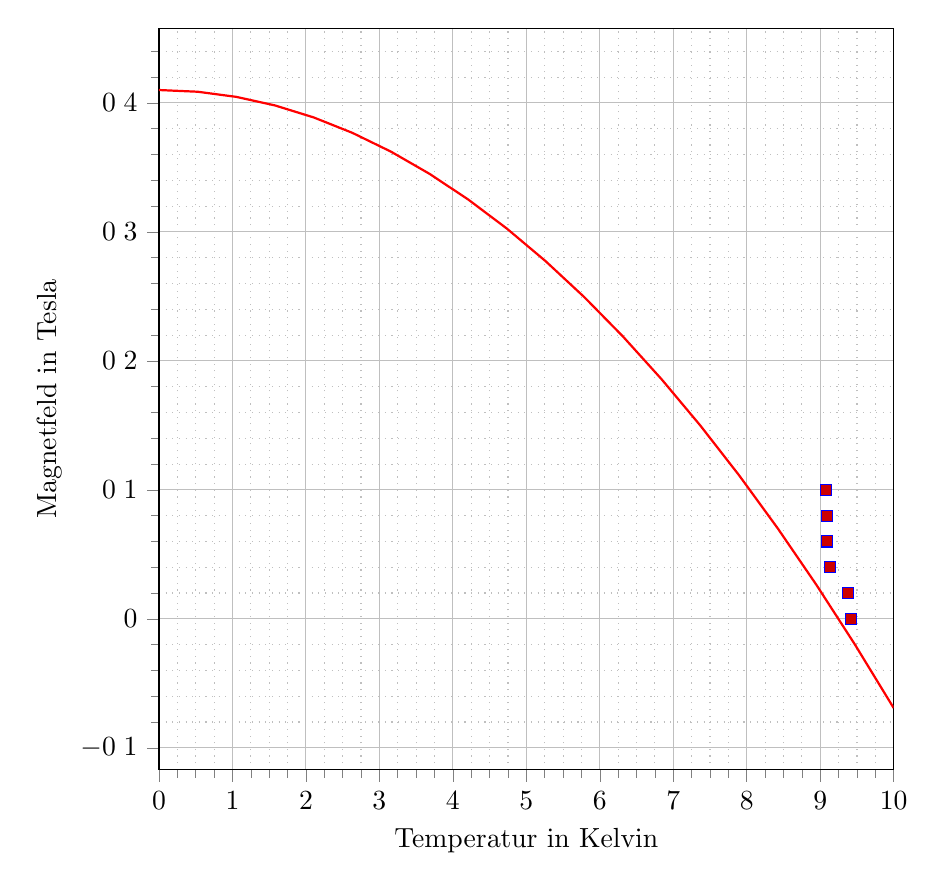
\begin{tikzpicture}
\begin{axis}[
    xlabel=Temperatur in Kelvin,
    ylabel=Magnetfeld in Tesla,
    width=0.9\textwidth,
    height= 11cm,
    xmin=0,
    xmax=10,
    grid=both,
    tick align=outside,
    tickpos=left,
    minor x tick num=3,
    minor y tick num=4,
    minor grid style={dotted,thin},
    scaled ticks=false,
    xlabel near ticks,
    ylabel near ticks,
]

\addplot[red, thick, mark size=0.0pt, samples=20, domain=0:10]{0.41*(1-(x/9.25)*(x/9.25))};
\addplot+[blue, only marks, error bars/.cd,
  x dir=both,x explicit,
  %x dir=both,x fixed=0.05
  ] coordinates{
  (9.4230,0)    +-(0.0176,0.0076)
  (9.3780,0.02) +-(0.0120,0.0110)
  (9.1281,0.04) +-(0.0325,0.0198)
  (9.0918,0.06) +-(0.0102,0.0083)
  (9.0943,0.08) +-(0.0199,0.0136)
  (9.0830,0.10) +-(0.0076,0.0030)
};
\end{axis}
\end{tikzpicture}
\captionof{figure}{Gemessene Werte für das kritische Magnetfeld und theoretischer Verlauf. Die Fehlerbalken der gemessenen Werte sind zu klein um dargestellt zu werden.}
\end{center}
\end{figure}
\chapter{Fazit}
Im vorausgegangenen Versuch wurde erfolgreich der Supraleitende Zustand von den zwei Messproben erreicht. Zusammenfassend kann man sagen, dass wir die Sprungtemperatur von der verwendeten \ch{YBa2Cu3O7}-Probe erfolgreich und mit einem relativ geringen Fehler von \(\frac{\Delta T_C}{T_C} < 0,3\% \) auf \(  T_C = \tol{90,5189}{0,2329}{0,0912} \ \mathrm{K}\) bestimmt haben.
Leider hat sich aber allem Anschein nach bei dem Experimentieren mit Niob ein Fehler eingeschlichen, weswegen wir die zugehörige Theorie in diesem Versuch nicht bestätigen konnten. Im Nachhinein ist es schwer zu sagen, was die genaue Fehlerursache war. Trotzdem hat der Versuch an sich sehr viel Spaß gemacht und war natürlich auch sehr lehrreich. So konnten wir zum ersten mal ein Versuch mit Temperaturen nahe dem absoluten Nullpunkt durchführen und dabei die Handhabung mit flüssigem Helium miterleben. Auch die in dem Versuch verwendeten Messmethoden waren neu und konnten uns neue Erkenntnisse Vermitteln.


%ENDE INHALT

\cleardoublepage{}
% Eintrag fürs Inhaltsverzeichnis

\newpage
\begin{thebibliography}{100}
  \bibitem{finnemore} D. K. Finnemore, T. F. Stromberg, and C. A. Swen- son, Superconducting properties of high-purity nio- bium, Phys. Rev. 149 231 (1966).
  \bititem{mappe} Literaturmappe zum Versuch aus der physikalischen Bibliothek
\end{thebibliography}


\cleardoublepage{}
% Eintrag fürs Inhaltsverzeichnis
% Abbildungsverzeichnis einfügen
\addcontentsline{toc}{chapter}{Abbildungsverzeichnis}
\listoffigures

\end{document}

